%%%%%%%%%%%%%%%%%%%%%%%%%%%%%%%%%%%%%%%%%%%%%%%%%%%%%%%%%%%%%%%%%%%%%%%%

%%% LaTeX Template for AAMAS-2021 (based on sample-sigconf.tex)
%%% Prepared by Natasha Alechina and Ulle Endriss (version 2020-08-06)

%%%%%%%%%%%%%%%%%%%%%%%%%%%%%%%%%%%%%%%%%%%%%%%%%%%%%%%%%%%%%%%%%%%%%%%%

%%% Start your document with the \documentclass command.
%%% Use the first variant below for the final paper.
%%% Use the second variant below for submission.

\documentclass[sigconf]{aamas} 
%\documentclass[sigconf,anonymous]{aamas} 

%%% Load required packages here (note that many are included already).

\usepackage[inline]{enumitem}

\usepackage{balance} % for balancing columns on the final page

%%%%%%%%%%%%%%%%%%%%%%%%%%%%%%%%%%%%%%%%%%%%%%%%%%%%%%%%%%%%%%%%%%%%%%%%

%%% AAMAS-2021 copyright block (do not change!)

\setcopyright{ifaamas}
\acmConference[AAMAS '21]{Proc.\@ of the 20th International Conference on Autonomous Agents and Multiagent Systems (AAMAS 2021)}{May 3--7, 2021}{London, UK}{U.~Endriss, A.~Now\'{e}, F.~Dignum, A.~Lomuscio (eds.)}
\copyrightyear{2021}
\acmYear{2021}
\acmDOI{}
\acmPrice{}
\acmISBN{}

%%%%%%%%%%%%%%%%%%%%%%%%%%%%%%%%%%%%%%%%%%%%%%%%%%%%%%%%%%%%%%%%%%%%%%%%

%%% Use this command to specify your EasyChair submission number.
%%% In anonymous mode, it will be printed on the first page.

\acmSubmissionID{???}

%%% Use this command to specify the title of your paper.

\title[Soft Maximin Approaches to MODM]{A soft maximin approaches to Multi-Objective Decision-making for encoding human intuitive values}

%% we can update this later as appropriate

%%% Provide names, affiliations, and email addresses for all authors.

\author{James Bond}
\affiliation{
  \institution{Secret Intelligence Service}
  \city{Vauxhall, London}}
\email{agent007@mi6.gov.uk}

\author{Ada Lovelace}
\affiliation{
  \institution{Analytical Engines, Inc.}
  \city{Ockham Park}
  \state{Surrey}}
\email{ada@analytical-engines.com}

\author{Alan M. Turing}
\affiliation{
  \department{Computing Machine Laboratory}
  \institution{Victoria University of Manchester}}
\email{amt@vum.ac.uk}

%%% Use this environment to specify a short abstract for your paper.

\begin{abstract}

Balancing multiple competing and conflicting objectives is an essential task for any artificial intelligence tasked with satisfying human values or preferences. Conflict arises both from misalignment between individuals with competing values, but also between conflicting value systems held by a single human. Starting with principles of loss-aversion (as in maximin decicions) and maximin, we designed a set of soft maximin function approaches to multi-objective decison-making. Benchmarking these functions in a set of previously-developed environments, we found that one new approach in particular, `split-function exp-log loss aversion', performs better than the thresholded alignment objective method, the state of the art described in \cite{vamplew_potential-based_2021}. We explore approaches to further improve multi-objective decision-making using soft maximin approaches.

%`cover a middle ground between the linear approach and a lexicographic approach - This is now explained in section 1.4 "Our proposed functions are in turn a compromise between a thresholded leximin and the linear MEU function - they are continuous functions, while still representing the loss aversion aspect as a kind of soft maximin approach."
\end{abstract}

%%% The code below was generated by the tool at http://dl.acm.org/ccs.cfm.
%%% Please replace this example with code appropriate for your own paper.


%%% Use this command to specify a few keywords describing your work.
%%% Keywords should be separated by commas.

\keywords{Auction Theory, Reinforcement Learning, Social Simulation}

%%%%%%%%%%%%%%%%%%%%%%%%%%%%%%%%%%%%%%%%%%%%%%%%%%%%%%%%%%%%%%%%%%%%%%%%

%%% Include any author-defined commands here.
         
\newcommand{\BibTeX}{\rm B\kern-.05em{\sc i\kern-.025em b}\kern-.08em\TeX}

%%%%%%%%%%%%%%%%%%%%%%%%%%%%%%%%%%%%%%%%%%%%%%%%%%%%%%%%%%%%%%%%%%%%%%%%

\begin{document}

%%% The following commands remove the headers in your paper. For final 
%%% papers, these will be inserted during the pagination process.

\pagestyle{fancy}
\fancyhead{}

%%% The next command prints the information defined in the preamble.

\maketitle 

%%%%%%%%%%%%%%%%%%%%%%%%%%%%%%%%%%%%%%%%%%%%%%%%%%%%%%%%%%%%%%%%%%%%%%%%

\section{Introduction}




A key aim of AI Safety research is to align AI systems to the fulfillment of human preferences \cite{Bostrom2014, russell2019human} or values. Prior commentary has described at least three reasons why this is a multi-objective (MO) problem. First, there are a variety of ethical, legal, and safety-based frameworks \cite{vamplew_human-aligned_2018}, and alignment to any one of these systems is insufficient. Second, even within a specific category--for instance, moral systems--there exist competing accounts of moral outcomes, including amongst philosophers of ethics and morality \cite{bogosian_implementation_2017}. Third, according to the moral intuitionist account of human moral cognition, moral cognition is a plural and contradictory set of social intuitions \cite{haidt2001emotional,sotala2016defining}.

Human values cannot be reliably reduced to a consistent single outcome or value function in any indisputable way. When a value is held for its intrinsic, axiomatic worth, quantifying trade-offs precisely is impossible. When conflicts between fundamental values occur, any possible solution will violate one or more values and be considered unsatisfactory.  

One solution is to design systems that aim for Pareto-optimality, but as the number of objectives increases, it becomes harder to achieve strict Pareto-optimality \cite{rolf_need_2020}. It may then be necessary to look for a heuristic solution that balances Pareto-optimality with the ability to achieve reasonable compromise between objectives. 
%Roland: Also, Pareto optimality provides only a boundary, a set of solutions. We further restrict this set of states to consider the fairness aspect as well.
% As I see it, at least in some cases our solution is a subset of Pareto optimality. In other words, Pareto optimality is still too undetermined and contains a too large set of possible states. 

%It can be argued that having multiple objectives, none of which is allowed to dominate over others, helps to mitigate against Goodhart's / Campbell's law as well. These laws manifest when a pressure is placed upon a particular measure or indicator and it becomes an objective. When the measures are somewhat uncorrelated and domination of any objective is forbidden by a utility aggregation function then particular measures are avoided from bearing too much pressure. 

\subsection{Current approaches}

\subsubsection{Multi-objective decision-making in reinforcement learning}
The inclusion of multiple objectives in reinforcement learning tasks was previously explored \cite{vamplew_human-aligned_2018,vamplew_potential-based_2021}  in the form of  \textit{maximin} approaches and \textit{leximin} approaches.
%Multiple-objective approaches have been previously explored  \cite{vamplew_human-aligned_2018,vamplew_potential-based_2021}
%\footnote{cite also earlier work/other work that we have not directly used? like 'classical' papers if MODM?}
%in reinforcement learning
%as functions for reinforcement learning
%\footnote{first talk about MODM then about RL}
%tasks.% when combining multiple objectives. 
%A particularly interesting context for this is low-impact AI \cite{vamplew_potential-based_2021}, where a \textit{primary objective} must be balanced against a \textit{secondary objective].
%not sure if the above is a necessary part of this narrative or not?
%These have included \textit{maximin} approaches and \textit{leximin} approaches.
A maximin approach aims to maximize the value of the lowest member of a set--for instance, the outcomes for the least-well-off person in a group of people \cite{rawls2001justice}. A maximin approach may also maximize the value of the least-optimized value (`objective' in a MO setting)--for instance, in the context of low-impact AI \cite{vamplew_potential-based_2021}, balancing across a safety objective
and a primary objective. A leximin approach orders a set of objectives, and then optimizes for the first value in the set, followed by the second value, and so on; a formal description can be found in \cite{vamplew_human-aligned_2018}.

\subsubsection{Non-linear multiple objective functions}
Non-linear utility functions have been previously explored in \cite{rolf_need_2020}. It was found that a non-linear objective system traversing a learning-space through reinforcement learning learns highly satisfactory solutions, balancing contradictory needs. That work followed earlier approaches that attempted to exhaustively explore \cite{van2014multi,parisi2016multi} a space or a subset thereof \cite{barrett2008learning} of Pareto-improvements to the current state space.

A multiple objective reward exponential function was proposed \cite{rolf_need_2020}, of the form:

\begin{align}\label{eq:rolf}
f(x)= &  -\exp(-x) \\ \nonumber
\end{align}

 where $x$ is untransformed reward signal, and $f(x)$ is a function that creates a `loss averse' transformation of the reward.

The methods section below introduces alternative multiple objective exponential functions and explains the bases for the deviations from the previously proposed \cite{rolf_need_2020} design as in Equation~\ref{eq:rolf}.

\subsubsection{AI Morality}

There has been at least one prior effort made to capture moral uncertainty in AI \cite{martinho_empirical_2020}. In this project, a discrete choice analysis model was used to demonstrate moral uncertainty about alternative policy choices.

%\subsubsection{Scaling}

%Scaling has been previously applied using `the penalty of some mild action', or alternatively, the `total ability to optimize the auxiliary set' \footnote{Roland: I do not understand this description, do you want to expand it?} \cite{turner_conservative_2020}, although in this account, a scale is applied across all reward functions. \footnote{why are we mentioning scaling? doesn't seem contextual here. should mention it but context needs to be described}

\subsubsection{Theoretical approaches}


`Conservative agency' has been previously described as a unification of side effect avoidance, state change minimization, and reachability preservation \cite{armstrong_low_2017, turner_conservative_2020}. Its goal is to optimize `the primary reward function while preserving the ability to optimize others', or `Attainable Utility Preservation'.
%Roland: This low-impact AI approach can also be technically implemented as a form of multi-objective AI.

Conservativism in Bayesian \cite{pmlr-v125-cohen20a} or neuromorphic systems \cite{byrnes_steve_conservatism_2020} has also been previously proposed, including the possibility of requesting help from an agent mentor.


%%%% Peter's provided a nice summary of a bunch of papers. I want to avoid filling this workshop paper up with a full review of the field--it's probably not necessary--but we should give the main prior accounts at least to explain why ours is different.


%%PV: "There’s the work by Saisubramanian et al which we cited in “Potential-based multiobjective reinforcement learning approaches to low-impact agents for AI safety”: Saisubramanian, S., Kamar, E., Zilberstein, S., 2020. A multi-objective approach to mitigate negative side effects. In: Proceedings of the Twenty-Ninth International Joint Conference on Artificial Intelligence."
%%PV: "Also the paper by Elfwing et al might interest you, given that it is based on psychology and neuroscience:  Elfwing, S., Seymour, B., 2017. Parallel reward and punishment control in humans and robots: Safe reinforcement learning using the maxpain algorithm. In: 2017 Joint IEEE International Conference on Development and Learning and Epigenetic Robotics (ICDL-EpiRob). IEEE, pp. 140–147."
%%PV: "This paper from IBM takes a somewhat multiobjective approach to building an ethical AI agent: Noothigattu, R., Bouneffouf, D., Mattei, N., Chandra, R., Madan, P., Varshney, K. R., ... & Rossi, F. (2019). Teaching AI agents ethical values using reinforcement learning and policy orchestration. IBM Journal of Research and Development, 63(4/5), 2-1."
%%PV: "Lastly the maximin approach is obviously closely tied to the concept of fairness. This is a nice paper which looks at a more general class of aggregation functions for fairness based on the Generalised Gini Social Welfare function. Siddique, U., Weng, P., & Zimmer, M. (2020, November). Learning Fair Policies in Multi-Objective (Deep) Reinforcement Learning with Average and Discounted Rewards. In International Conference on Machine Learning (pp. 8905-8915). PMLR."




%\subsection{orphaned sections}

%(these are isolated points that probably need to be made; I'm not sure where tehy should be a this point).

%(do we need to briefly discuss the distinction between thinking about MORL and MO decision-making? probably doesn't need discussion but we need to make sure the disinction is kept clear in our own text)

%Go back and discuss core ideas and motivations--do we mention using a min function with decision paralysis? My progress has been something like a realization that decision-paralysis will happen very quickly; what do we do then? This paper tries to address that question.

%- Roland: I propose to leave decision paralysis out of this paper.Decision paralysis seems to be a quite interesting and deep topicfor me. Maybe it is easier to start illustrating it with a paralysisbetween two performance objectives. Paralysis between a safetyobjective and a performance objective may not be so clear cut casesince doing nothing might be the safest thing, and therefore needsmore complex analysis than the paralysis between two performanceobjectives

%(subagent solution for wireheading: In order to prevent wireheading, I propose a multi-objective agent with objective functions determined by subagents run on observation-utility maximization \cite{dewey_learning_2011}. Each subagent is somehow primed to respond to a particular moral objective, perhaps with an objective function that maximizes for a particular value.)
%--out of scope, but Ben Smith should follow this stuff up I guess?

%(make sure we discuss applications in terms of Victoria Krakovna's of problems and/or DeepMind's scenarios and how MORL is important for resolving these, making sure that no objectives get ignored in the context of AI, distinct from AGI--Roland to add this?)
%Roland: This too seems to be appropriate for the next paper since we did not cover stronger multi-objective cases there, where there are two or more safety objectives or two or more performance objectives.

%(This section includes references to various prior literature and directions that need to be explored before we submit this paper.)


%\subsubsection{}
%Preferences are often, but not exclusively, expressed in negative terms--limits on behavior that produces undesirable outcomes rather than prescriptive desirable outcomes. 

%\subsection{Prior work for editing}


\subsection{Building on previous work}

This paper is the first to examine continuous non-linear multi-objective decision-making in the context of low-impact AI work as described in \cite{vamplew_potential-based_2021}. It is also the first we are aware of to apply a split-function exponential-log transform to any AI decision-making or RL application.  Previous work has explored continuous functions for traversing environments where rewards need to be gathered in different parts of the environment and traded off over time \cite{rolf_need_2020}, although that work focused on a function resembling ELA and did not explore SFELLA (these are described below). 

\cite{turner_conservative_2020} started out with similar goals to ours; they described `conservative agency' to balance `optimization of the primary reward function with preservation of the ability to optimize auxiliary reward functions'. They did not examine non-linear combinations of objectives, and instead focused on learning approaches for optimizing the scaling between objectives. We have not applied arbitrary scaling between objectives, and applying the scaling method as in \cite{turner_conservative_2020} could be complementary to our work.


\subsection{Pluralistic human value system}

Often, AI alignment aims to ensure AI systems fulfill human preferences. While neither human preferences nor human values are always consistent \cite{sotala2016defining}, values are higher-order and harder to identify \cite{barrett2008learning}, but preferences are more sensitive to context and recalculation \cite{warren2011values}. The framework here focuses on modeling distinct human values as distinct objectives, while recognizing that there may be many preferences to satisfy within each overarching value function. As outlined above, intuitions of individuals frequently conflict \cite{haidt2001emotional} and moral views between individuals also conflict \cite{bogosian_implementation_2017}.

It has been argued that one way to address uncertainty in moral decision-making is to learn human moral judgement in a bottom-up fashion \cite{bogosian_implementation_2017}; rather than learning human values, an agent learns human preferences, and those preferences are implicitly held within values. Even if this is technically adequate, in practice it might be necessary to put constraints on system to ensure they don't learn anti-social preferences \cite{neff2016talking}.

%This approach been challenged: creators of AI systems may themselves have disagreement about what counts as `moral', and will need to make choices about the way systems are designed  \cite{bogosian_implementation_2017}. For this reason, it's likely the bottom-up approach will be considered insufficient, and attempts will be made to correct the system \cite{stray2020you}, either by re-engineering the learning approach or through post-hoc correction. For instance, we may expect an AI system to rise above human racial prejudices rather than reflect them. 

Furthermore, a utility function based on human preferences themselves has been argued to be an insufficient definition of value \cite{sotala2016defining, DBLP:journals/corr/abs-1712-05812}, because \begin{enumerate*}
    \item humans do not have consistent utility functions,
    \item utility functions are poor models of conflicts between lower- and higher-order preferences,
    \item it fails to draw distinctions between `wanting' and `liking', and
    \item a utility function of unitary value could not adequately generalize from existing values to new ones.
\end{enumerate*}

It is also an important question of how to combine the rewards that are based on human preferences. The proper way should not be a trivial sum of the individual rewards since that would skip the nonlinear transformation by the utility functions before the final aggregation takes place. Nonlinear utility functions are in fact commonly used in single
objective settings \cite{rolf_need_2020} therefore they naturally need to be used in multi-objective setting as well.

A theoretical Bayesian preference-learning system could model preferences and through learning human values, learn the proper way to combine them. But there is the trade-off between a model being too simple (linear sum of rewards), and too complex (a Bayesian network, requires potentially unpractical amounts of data). The middle ground would be to have a model-based approach which describes some rules (like the presence of negative exponential shape for violated alignment objectives) while being still flexible and able to learn the data as parameters of the model.
%\footnote{I have to say, now that I have looked at this argument, I think it is fairy weak. I think a stronger challenge to the unitary preference learning approach, as advocated by Stuart Russell, is Kyle Bogosian's approach above; however I am not entirely convinced by that either. Something to add to the `limitations' section perhaps}





%\subsection{Conflicting individual preferences}\footnote{Roland: Is there missing something? Section 1.4 seems to follow immediately?}

\subsection{Design principles}
% TODO: look at Roland's desiderata file and make sure stuff is covered
%\footnote{avoid breaking after the section header!}
%Roland: TODO: The desiderata file is still missing some core ideas or clarity, need to fix that sometime.
The following principles guided us in selecting an aggregate function different to the maximin or leximin approaches:
\begin{enumerate}
    \item \textit{Loss aversion}, \textit{conservatism}, or \textit{soft maximin}. We seek to improve the position of the lowest member of the set of values, while also not entirely disregarding optimization of other values.
    \item \textit{Balancing outcomes across objectives}. %There are at least two different ways to distinguish separate objectives; balancing outcomes across objectives is important in both cases. 
    Each objective represents a different moral system, each moral system bears some non-zero probability of being correct. To be conservative and ensure a low probability of any bad outcome, we avoid strongly negative outcomes in any system. Alternatively, each objective represents a particular subject's preferences. Then, balancing outcomes across objectives represents an implementation of fairness between subjects.
    \item \textit{Zero-point consistency}. An agent evaluates whether an action performs better not only compared to alternatives, but also compared to no action at all, which would have a value of 0. For this reason any aggregation or transformation function should preserve the overall estimated sign or valence of an objective.
\end{enumerate}

Previous work \cite{vamplew_potential-based_2021} has described thresholded leximin approaches in order to trade-off objectives, in the context of trading off a Primary objective and an Impact Objective in low-impact AI. A thresholded leximin function aims to first maximize the thresholded value of thresholded objectives, and then secondarily maximize the unthresholded value of one or more other objectives. If the alignment objective is thresholded, then the system aims to first achieve at least a thresholded level of the alignment objective, and then subject to this, to achieve a maximum level of the performance objective. Alternatively, a \textit{complete thresholded leximin}, aims to maximize the thresholded value of all objectives, i.e., reach the threshold on each objective; then, subject to this, aims to maximize the unthresholded value of each objective.

This complete thresholded leximin is a discretely-stepped maximin approximation. Reaching a specified minimum threshold value on each objective takes precedence over maximizing already-high values. Yet it is not a strict maximin, because the function doesn't only care about maximizing the minimum value; in fact, beyond a specified threshold, no value is given at all. In this way a thresholded leximin can be seen as a compromise between a maximin function and a linear maximum expected utility (MEU) function.

\subsection{Current proposal} 
In this paper we propose another compromise between a maximin and a linear MEU function: here, following previous work \cite{rolf_need_2020}, we propose a continuous rather than discrete trade-off between maximin and linear MEU. This approach avoids specifying a threshold, which may be desirable for at least three reasons. First, it might not be possible to specify an appropriate threshold in advance. Second, continuously decreasing the extent to which we prioritize an objective might better fit our underlying aims or values than giving a high priority up to a threshold and no priority at all above that threshold. %A continuous compromise would continue to prioritize maximizing the least maximal values, giving decreasing weight to this as the value increases but not switching its priority entirely in a stepped fashion at any point. 
Third, in the context of modeling human values, this approach might sometimes be more consistent with human value processing\cite{Tom515}, considering the literature on risk aversion \cite{pratt1978risk}.


A continuous compromise between multiple values using non-linear multiple objective systems also offers greater benefits for complex low-impact artificial systems. If one had dozens of objectives, a strict maximin or leximin function might come to be overly inflexible. In order to be low-impact, a system must evaluate the specific, counterfactual impact of its own actions on those states. If a system with dozens of competing objectives evaluated the effect of its own actions on the state of the world, and `no action' was one possible choice, there is a high probability that most of the time, `no action' would win, because of the high likelihood that every possible action evaluates negatively according to some function. A soft maximin function that combines MEU with a strong penalty for negative utility might facilitate more action without substantially increasing risk.


\section{Method}
We adapted algorithms in \cite{vamplew_potential-based_2021}, comparing the existing $TLO^A$ aggregation function with several new aggregation and scalarization functions. These were compared using the same environments and benchmarks as in \cite{vamplew_potential-based_2021}. Specifically, the environments were the UnbreakableBottles environment, the BreakableBottles environment, the Sokoban Environment, and the Doors environment.
\subsection{Testing environment}

We used a modified version of the testing environment from \cite{vamplew_potential-based_2021}, obtained with permission from the authors. Learning proceeded for 5,000 episodes, and performance during learning (online performance) and after learning (offline performance) was measured. There were several key changes for our implementation. Changes affecting modeling results themselves are described below.



\subsection{Aggregation functions}



All of the multi-objective utility functions we compared work as follows. 
\begin{enumerate}

    \item Apply an objective specific scaling factor $c_i$ which is multiplied with the value of the reward. Different objectives likely have different scaling factors.  
    \item Transform the scaled output using a non-linear transform (Figure~\ref{fig:transform_functions} and Figure ~\ref{fig:seba_transform_functions_3d}). %For SFMLA, SFELLA, ELA, LELA, and SEBA, the transform is applied independently for each objective. % this is for ALL of the studied functions, right?
    
    \item Combine the transformed output using a simple average/sum.
\end{enumerate}

These steps describe a value function which can be applied either to the individual rewards of each time-step or to the values of the Q-values. In our current setup we applied the functions to the Q values.

Each non-linear function is applied component-wise before aggregation occurs by averaging/summing of the transformed values

\begin{align}
\label{eq:meu}
U=\sum_{i}^n{f_i(c_i x_i)}
\end{align}

\noindent where ${f_i}$ describes a specific transform function for the $i$th objective. Note that here, $U$ describes our modeling of Q-values. The scaling factors $c_i$ can be treated as parameters of the model. They could be, for example, specified directly by the human, automatically determined in the future by the agent using a value learning method, or calculated by some other algorithm. 
For the purposes of this experiment, we left these at $c=1$ (instead, we directly modified $x$, the value returned by the environment), but emphasize that modifying these scale values could be useful in the future.


 New non-linear transforms compared are:

\begin{itemize}
    %\item Split-function multiplicative loss aversion (SFMLA)
    \item Split-function exp-log loss aversion (SFELLA)
    \item Exponential loss aversion (ELA)
    \item Linear-exponential loss aversion (LELA)
    \item Squared error based alignment (SEBA)
\end{itemize}

\noindent The SEBA transform function envisages differing functions for two categories of objectives. All other transform functions do not distinguish categories of objectives, and apply the same function over all objectives.

Each non-linear transform is a transform of the value obtained along a specific objective %$O$
at a specific state %$s$ 
with a specific action %$a$\footnote{need to decide how much of this notation we include. If we include it, need to rewrite formulae to reflect it. Might take some inspiration from Vamplew's earlier papers. Should almost certainly be giving a formula for $TLO^A$}. 
The SFELLA, ELA, and LELA functions are illustrated in Figure~\ref{fig:transform_functions}. The SEBA aggregation is illustrated on Figure ~\ref{fig:seba_transform_functions_3d}.

For each transform, where $x=0$, $f(x)=0$. This is a minor modification from the non-linear transform previously proposed in \cite{rolf_need_2020}, typically achieved by adding 1 to the outcome value.

Each function also provides that $\frac{\mathrm{d} f(x) }{\mathrm{d} x}$ declines as $x$ gets larger. This lowers inequality between outcomes as measured in different objectives, objectives where values are strongly negative get disproportionately higher priority. Where different objectives were operationalizing, for instance, priorities among different interested parties, this might be particularly useful in reducing inequality between outcomes.



\begin{figure*}[h]
 
  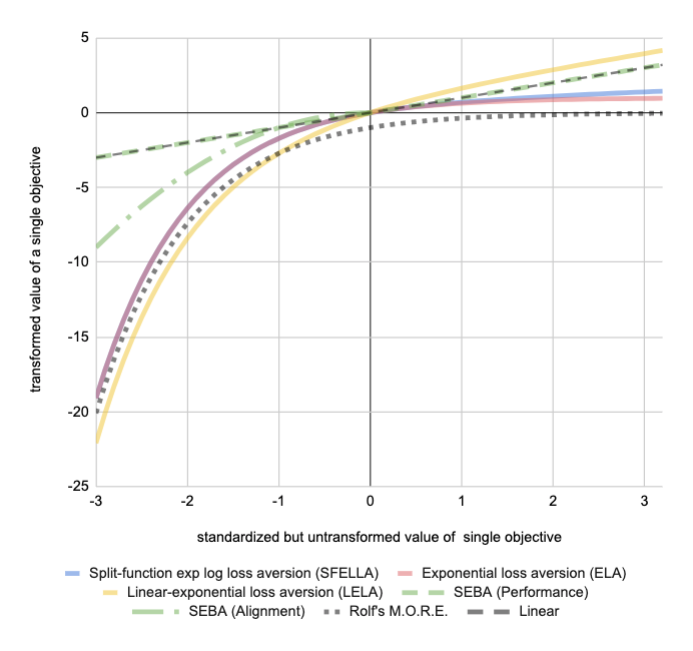
\includegraphics[width=\columnwidth]{output/transform_graph-2d_with_rolf2.png}%\footnote{Roland: Can you please add the -x*x from SEBA to the left part of the plots too? Maybe using some short-dashed line for example. It would illustrate that the square function is less steep than the exponential functions, thus being in between linear and exponential}
  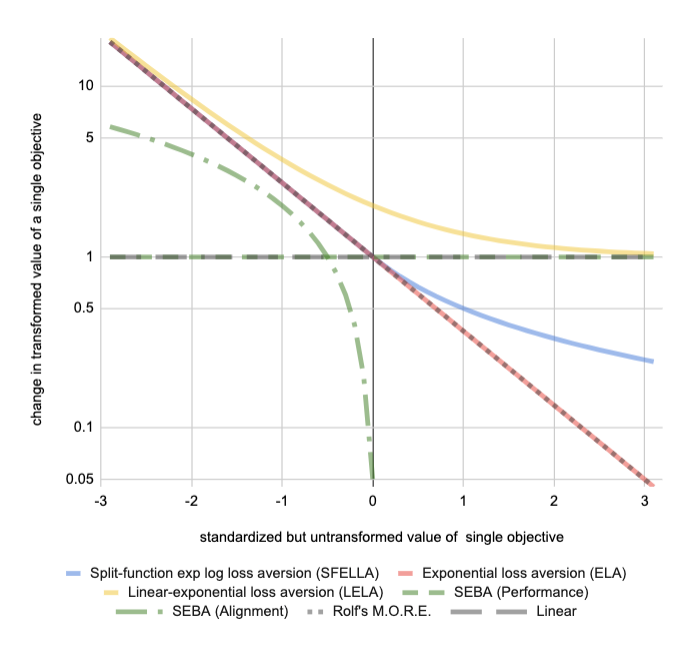
\includegraphics[width=\columnwidth]{output/transform_graph_2d_integral_with_rolf2.png}%\footnote{Roland: I would add comment that the the y scale is log scale, otherwise this plot is confusing, until one looks at the numbers at the left side}
  \caption{Transform functions. Left: Each transform function is applied to the reward received from the environment for each objective, or to the Q value of the RL agent for each objective. In our current setup it is applied to the Q values of the RL agent.
  %\footnote{why repeat the same thing when you can leave out the other option?}. 
  The output of each of these transform functions are averaged together % in a Maximize Expected Utility Model \footnote{if anything this should be called MOMEU, right?}
  (Equation~\ref{eq:meu}). Right: Change in $f(x)$ per unit $x$, with $y$ axis plotted on a log scale%\footnote{could be omitted}
  . Note that ELA and SFELLA produce greater-than-linear change in $f(x)$ when $x<0$ and less-than-linear change when $x>0$. In contrast, LELA's change never falls below 1.}
  \label{fig:transform_functions}
  \Description{Transform functions.}
\end{figure*}

\begin{figure*}[h]
 
  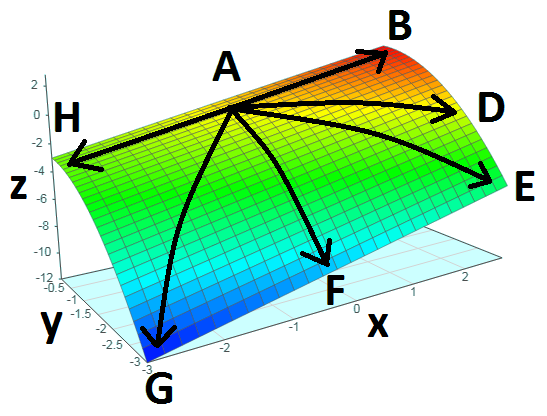
\includegraphics[width=\columnwidth]{output/seba1b.png}
  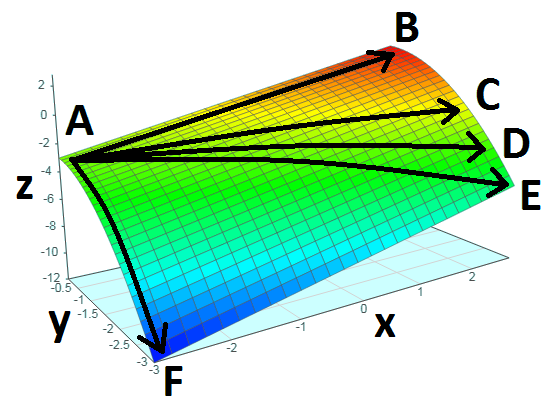
\includegraphics[width=\columnwidth]{output/seba2b.png}
  \caption{Transform for the SEBA aggregation. One of the objectives is the alignment objective (the y-axis), and the other objective is the performance objective (the x-axis). The z-axis represents the aggregated utility. The two types of objectives are treated differently. The performance objective has always linear treatment regardless of the current sign of its input measure, while the alignment measure is upper-bounded at zero and has exponential treatment (in case of SEBA it is a negated squared error). These plots illustrate two things. 1. The performance objective (the x-axis) is linear regardless of the sign of the value of the input measure. 2. The alignment related measure (the y-axis) may be sacrificed, but only up to a degree. Once alignment would be sacrificed too much, the evaluation of the aggregated utility quickly becomes strongly negative, since the alignment measure is treated exponentially. So this provides the loss aversion aspect.}
  \label{fig:seba_transform_functions_3d}
  \Description{Transform for the SEBA aggregation.}
\end{figure*}

%SFMLA might be the function that most intuitively expresses loss aversion, the idea that losses loom larger than gains:

%\begin{align}
%U^P(s, a)'= & cU^P(s, a) & \mathrm{ where \: U^P(s, a)>0} \\ \nonumber
%  &  2c U^P(s, a) &  \mathrm{otherwise} \\ \nonumber
%\end{align}

%(or we can write the following; which is better?)

%\begin{align}
%f(x)= & cx & \mathrm{ where \: x>0} \\ \nonumber
%  & 2c x &  \mathrm{otherwise} \\ \nonumber
%\end{align}

In SFELLA, there is a split in the function at $x=0$. It expresses a loss-averse function where losses will be amplified more than gains:

\begin{align}
f(x)= & \ln(cx+1) & \mathrm{ where \: x>0} \\ \nonumber
  &  -\exp(-cx)+1 &  \mathrm{otherwise} \\ \nonumber
\end{align}

Additionally, by implementing a log rather than a negative exponential in the positive domain, the function retains relatively more weight on positive objectives, i.e. is not bounded.

The ELA is a simplification of this without a case distinction at the cost of giving very little weight to any increase in values over 1:

\begin{align}
f(x)= &  -\exp(-cx)+1 \\ \nonumber
\end{align}

With LELA we add a $x$ term so that value continues to increase at least linearly for large inputs:

\begin{align}
f(x)= &  -\exp(-cx)+cx+1 \\ \nonumber
\end{align}

This still yields loss aversion at points less than zero but always provides that an increase in $x$ increases at least linearly in $f(x)$%\footnote{sound repetitive}.


Finally, SEBA implements a different set of principles. Instead of branching depending on the value of $x$ the function treats the dimensions differently depending on their type: depending on whether a dimension is part of the performance objective or part of the alignment objective.%\footnote{earlier this was called a safety objective}.

For performance objectives the SEBA formula is linear:
\begin{align}
f(x)= &  cx \\ \nonumber
\end{align}
There is no differentiation between negative and positive areas of the measures of the performance objectives. This avoids the need for establishing a zero-point. Proper scaling is still needed.

For alignment objectives the SEBA formula is a negated square power function in order to express loss aversion. It is assumed that the incoming rewards in the alignment objective can only be negative or zero.
\begin{align}
\label{eq:seba}
f(x)= &  -(cx)^2 \\ \nonumber
  &  \mathrm{ where \: x \leq 0}
\end{align}
The alignment related measures still have a “natural” zero-point, since they by definition are bounded at zero where no (soft) constraint violations are occurring. Therefore in case of safety related features it is not so difficult to establish where the zero-point is located at. Such measures would usually measure the deviation of something from a desired target value. Such measures have two main types:
\begin{itemize}
    \item The desired target value is zero (for example, zero harm, etc).
    \item Alternatively it might be a homeostatic set-point (for example, optimal temperature, etc), so the measure is representing the negated absolute value of the deviation regardless of the direction of the deviation.
\end{itemize}
The SEBA aggregation is illustrated on Figure ~\ref{fig:seba_transform_functions_3d}. A number of specific situations are illustrated in the graph using upper-case letter points, and it is helpful to consider their interpretation:
  \begin{itemize}
      \item A - The initial state. The alignment objective / soft constraint is met and the performance objective is either at zero (left side plot) or at negative value (right side plot).
      \item B - The performance objective is improved, the alignment constraint is preserved. Moving in this direction changes the aggregated score linearly thus enabling independence from the zero-point.
      \item C - Shown only on the right side plot. Performance objective is improved significantly, while alignment constraint is sacrificed just so slightly that the aggregated utility is still improved.
      \item D - Performance objective is improved significantly, but the alignment constraint is sacrificed so much that the aggregated utility does not change as compared to the initial state. The agent is neutral to this state change and is not driven towards this state nor avoiding it.
      \item E - Performance objective is improved significantly, while the alignment constraint is violated significantly. Therefore the aggregated utility becomes worse than the initial state. The agent avoids this state.
      \item F - The measure for the performance objective does not change, but the alignment constraint gets violated.
      \item G - Shown only on the left side plot. Both the performance objective and the alignment objective / constraint get worse.
      \item H - Shown only on the left side plot. The performance objective gets much worse but the alignment constraint is still satisfied. It is also noteworthy that this state is evaluated to be about as good as the alternative state somewhere between D and E where the alignment constraint is getting notably violated but the performance objective is improved much.
  \end{itemize}

\subsection{Environment}

In every environment, agents have two objectives: a `performance' objective and an `alignment' objective. %\footnote{need to standarize terms. are we using primary or performance or reward; impact or alignment or penalty; etc - Roland: I vote for performance objective and alignment objective. These terms are in use also in Vamplew's code. It seems to be also important to avoid using the phrase "primary" objective as it is quite misleading in our context, since in practice the alignment objective is stronger and therefore sort of more primary. The word "reward" can remain where it is appropriate, since it is a measure, a proxy for the objective.} 
We started with four environments reported in \cite{vamplew_potential-based_2021}. We wanted to understand how different aggregation functions could respond to perturbations in goal magnitudes / scaling factors. To do this, we repeated each experiment 9 times. The first time was with the original settings as in \cite{vamplew_potential-based_2021}. Then, we repeated this with each environment's Performance reward feedback scaled by $10^{-2}$, $10^{-1}$, $10^1$, and $10^2$. The same range of scaling was then applied to the Alignment reward feedback. This scaling could in some scenarios potentially be distinguished from $c$ in Equations~\ref{eq:meu}-\ref{eq:seba}. Even though it is mathematically equivalent in our implementation, it could represent changes to the environment rather than changes in agent evaluation.

\subsection{Benchmark}

Each of the proposed functions was compared against the best performing function in \cite{vamplew_potential-based_2021}, the `TLO$^A$' function, on the `R$^*$' metric from the same paper. The `R$^*$' arbitrarily scores a weighted combination of Performance and Alignment objectives where one unit of Alignment objective (always on a negative scale) is worth 10-50 units of the Performance objective, depending on the environment.%\footnote{Roland: The ratio of units is somewhat different across environments. It is not always 50 units. Vamplew paper describes the details. I think the range was about 10 to 50.}



\section{Results}
Learning was switched off after 5000 episodes. Following that time, offline performance was observed. There was very little difference between the best-performing proposed function and $TLO^A$. For this reason, the remainder of the results reported will discuss performance during online testing, i.e., performance during learning itself.% and Offline testing\footnote{did we meantion what those words mean, did we even mention learning before?}. 


\begin{table}[t]
\footnotesize
  \caption{Mean $\text{R}^*$ Online performance. Each row represents comparable performance across 5 different objective functions. Values within 10\% of the best value in each row are highlighted. Higher scores are better. Items are significantly different from $\text{TLO}^A$ when marked *$p<0.05$, ** $p <0.01$, *** $p<0.001$.}
  \label{tab:mean_r_star_performance}
%\begin{adjustbox}{width=\columnwidth,center}%
%\resizebox{\textwidth}{!}{
\begin{tabular}{>{\raggedright\arraybackslash}p{5em}>{\raggedleft\arraybackslash}p{4em}>{\raggedright\arraybackslash}p{4.5em}rrrrr}
\toprule
Environment & Objective Modified & Objective Scale & EEBA1 & ROLF_EXP_LOG1 & SEBA & SFELLA & TLO$^A$\\
\midrule
 &  & 1 & 1.40** & 4.08*** & \textcolor{black}{1.43**} & \textcolor{blue}{6.54***} & \textcolor{black}{1.81}\\
\cmidrule{2-8}
 &  & 0.01 & 1.27 & 4.39*** & \textcolor{black}{1.33} & \textcolor{black}{1.38} & \textcolor{black}{1.46}\\

 &  & 0.1 & 1.38 & 4.21*** & \textcolor{black}{1.39} & \textcolor{black}{1.88**} & \textcolor{black}{1.41}\\

 &  & 10 & 6.08*** & 3.45*** & \textcolor{blue}{6.32***} & \textcolor{black}{4.44***} & \textcolor{black}{-0.22}\\

 & \multirow[t]{-4}{4em}{\raggedleft\arraybackslash Alignment} & 100 & -7.12*** & -4.08*** & \textcolor{blue}{2.22***} & \textcolor{black}{-3.49***} & \textcolor{black}{-0.48}\\
\cmidrule{2-8}
 &  & 0.01 & 5.85*** & 5.45*** & \textcolor{blue}{6.34***} & \textcolor{black}{5.51***} & \textcolor{black}{1.96}\\

 &  & 0.1 & 5.89*** & 5.38*** & \textcolor{black}{2.46**} & \textcolor{blue}{6.43***} & \textcolor{black}{1.88}\\

 &  & 10 & 1.50* & -14.73*** & \textcolor{black}{1.41**} & \textcolor{blue}{6.51***} & \textcolor{black}{1.77}\\

\multirow[t]{-9}{5em}{\raggedright\arraybackslash Breakable Bottles} & \multirow[t]{-4}{4em}{\raggedleft\arraybackslash Performance} & 100 & 1.48* & -12.83*** & \textcolor{black}{1.46**} & \textcolor{blue}{6.40***} & \textcolor{black}{1.81}\\
\cmidrule{1-8}
 &  & 1 & 1.47*** & -9.33*** & \textcolor{black}{-0.48***} & \textcolor{blue}{4.38***} & \textcolor{black}{3.87}\\
\cmidrule{2-8}
 &  & 0.01 & -0.76** & -9.34*** & \textcolor{black}{-0.73*} & \textcolor{black}{-0.58} & \textcolor{black}{-0.49}\\

 &  & 0.1 & -0.54 & -9.32*** & \textcolor{black}{-0.64} & \textcolor{blue}{8.29***} & \textcolor{black}{-0.63}\\

 &  & 10 & 3.53 & -9.71*** & \textcolor{blue}{3.43} & \textcolor{blue}{3.74} & \textcolor{blue}{3.63}\\

 & \multirow[t]{-4}{4em}{\raggedleft\arraybackslash Alignment} & 100 & 3.59*** & -9.88*** & \textcolor{black}{3.16**} & \textcolor{black}{2.73} & \textcolor{black}{2.82}\\
\cmidrule{2-8}
 &  & 0.01 & 3.70** & 3.59*** & \textcolor{black}{3.43***} & \textcolor{black}{3.66***} & \textcolor{blue}{4.09}\\

 &  & 0.1 & 4.36*** & 3.67* & \textcolor{blue}{5.39***} & \textcolor{black}{4.10} & \textcolor{black}{3.91}\\

 &  & 10 & -0.40*** & -14.18*** & \textcolor{black}{-0.70***} & \textcolor{blue}{4.41***} & \textcolor{blue}{3.97}\\

\multirow[t]{-9}{5em}{\raggedright\arraybackslash Doors} & \multirow[t]{-4}{4em}{\raggedleft\arraybackslash Performance} & 100 & -0.71*** & -13.75*** & \textcolor{black}{-0.51***} & \textcolor{blue}{4.17**} & \textcolor{blue}{3.85}\\
\cmidrule{1-8}
 &  & 1 & -15.03*** & 5.28*** & \textcolor{black}{-14.98***} & \textcolor{black}{-10.29***} & \textcolor{blue}{10.76}\\
\cmidrule{2-8}
 &  & 0.01 & -14.99 & 2.81*** & \textcolor{black}{-15.02} & \textcolor{black}{-14.97} & \textcolor{black}{-14.97}\\

 &  & 0.1 & -15.00 & 4.80*** & \textcolor{black}{-14.96} & \textcolor{black}{-14.98} & \textcolor{black}{-14.95}\\

 &  & 10 & 10.89*** & 3.43*** & \textcolor{blue}{10.88***} & \textcolor{blue}{10.92***} & \textcolor{blue}{10.72}\\

 & \multirow[t]{-4}{4em}{\raggedleft\arraybackslash Alignment} & 100 & 3.55*** & -0.10*** & \textcolor{blue}{10.82***} & \textcolor{black}{3.76***} & \textcolor{blue}{10.49}\\
\cmidrule{2-8}
 &  & 0.01 & 10.83 & 10.86* & \textcolor{blue}{10.91***} & \textcolor{blue}{10.86*} & \textcolor{blue}{10.77}\\

 &  & 0.1 & -14.99*** & 10.82 & \textcolor{black}{-14.96***} & \textcolor{black}{5.97***} & \textcolor{blue}{10.82}\\

 &  & 10 & -15.00*** & -5.30*** & \textcolor{black}{-15.01***} & \textcolor{black}{-11.05***} & \textcolor{blue}{10.88}\\

\multirow[t]{-9}{5em}{\raggedright\arraybackslash Sokoban} & \multirow[t]{-4}{4em}{\raggedleft\arraybackslash Performance} & 100 & -14.96*** & -6.69*** & \textcolor{black}{-14.96***} & \textcolor{black}{-10.97***} & \textcolor{blue}{10.82}\\
\cmidrule{1-8}
 &  & 1 & 28.70*** & 16.35*** & \textcolor{blue}{28.71***} & \textcolor{blue}{27.99***} & \textcolor{blue}{27.09}\\
\cmidrule{2-8}
 &  & 0.01 & 28.76 & 16.82*** & \textcolor{blue}{28.70} & \textcolor{blue}{28.73} & \textcolor{blue}{28.79}\\

 &  & 0.1 & 28.75 & 16.51*** & \textcolor{blue}{28.72} & \textcolor{blue}{28.74} & \textcolor{blue}{28.72}\\

 &  & 10 & 27.15*** & 15.81*** & \textcolor{blue}{27.62***} & \textcolor{blue}{25.90***} & \textcolor{black}{23.37}\\

 & \multirow[t]{-4}{4em}{\raggedleft\arraybackslash Alignment} & 100 & 25.27*** & 14.91 & \textcolor{blue}{25.66***} & \textcolor{black}{18.67***} & \textcolor{black}{14.60}\\
\cmidrule{2-8}
 &  & 0.01 & 27.04 & 26.75** & \textcolor{blue}{27.73***} & \textcolor{blue}{26.79*} & \textcolor{blue}{26.98}\\

 &  & 0.1 & 28.61*** & 26.48*** & \textcolor{blue}{28.66***} & \textcolor{blue}{27.82***} & \textcolor{blue}{27.15}\\

 &  & 10 & 28.70*** & 7.50*** & \textcolor{blue}{28.78***} & \textcolor{blue}{27.91***} & \textcolor{blue}{27.10}\\

\multirow[t]{-9}{5em}{\raggedright\arraybackslash Unbreakable Bottles} & \multirow[t]{-4}{4em}{\raggedleft\arraybackslash Performance} & 100 & 28.69*** & 16.01*** & \textcolor{blue}{28.75***} & \textcolor{blue}{27.85***} & \textcolor{blue}{27.08}\\
\bottomrule
\end{tabular}
}

\begin{tabular}{>{\raggedright\arraybackslash}p{5em}>{\raggedleft\arraybackslash}p{4em}>{\raggedright\arraybackslash}p{4.5em}rrrrr}
\toprule
Environment & Objective Modified & Objective Scale & EEBA1 & ROLF_EXP_LOG1 & SEBA & SFELLA & TLO$^A$\\
\midrule
 &  & 1 & 1.40** & 4.08*** & \textcolor{black}{1.43**} & \textcolor{blue}{6.54***} & \textcolor{black}{1.81}\\
\cmidrule{2-8}
 &  & 0.01 & 1.27 & 4.39*** & \textcolor{black}{1.33} & \textcolor{black}{1.38} & \textcolor{black}{1.46}\\

 &  & 0.1 & 1.38 & 4.21*** & \textcolor{black}{1.39} & \textcolor{black}{1.88**} & \textcolor{black}{1.41}\\

 &  & 10 & 6.08*** & 3.45*** & \textcolor{blue}{6.32***} & \textcolor{black}{4.44***} & \textcolor{black}{-0.22}\\

 & \multirow[t]{-4}{4em}{\raggedleft\arraybackslash Alignment} & 100 & -7.12*** & -4.08*** & \textcolor{blue}{2.22***} & \textcolor{black}{-3.49***} & \textcolor{black}{-0.48}\\
\cmidrule{2-8}
 &  & 0.01 & 5.85*** & 5.45*** & \textcolor{blue}{6.34***} & \textcolor{black}{5.51***} & \textcolor{black}{1.96}\\

 &  & 0.1 & 5.89*** & 5.38*** & \textcolor{black}{2.46**} & \textcolor{blue}{6.43***} & \textcolor{black}{1.88}\\

 &  & 10 & 1.50* & -14.73*** & \textcolor{black}{1.41**} & \textcolor{blue}{6.51***} & \textcolor{black}{1.77}\\

\multirow[t]{-9}{5em}{\raggedright\arraybackslash Breakable Bottles} & \multirow[t]{-4}{4em}{\raggedleft\arraybackslash Performance} & 100 & 1.48* & -12.83*** & \textcolor{black}{1.46**} & \textcolor{blue}{6.40***} & \textcolor{black}{1.81}\\
\cmidrule{1-8}
 &  & 1 & 1.47*** & -9.33*** & \textcolor{black}{-0.48***} & \textcolor{blue}{4.38***} & \textcolor{black}{3.87}\\
\cmidrule{2-8}
 &  & 0.01 & -0.76** & -9.34*** & \textcolor{black}{-0.73*} & \textcolor{black}{-0.58} & \textcolor{black}{-0.49}\\

 &  & 0.1 & -0.54 & -9.32*** & \textcolor{black}{-0.64} & \textcolor{blue}{8.29***} & \textcolor{black}{-0.63}\\

 &  & 10 & 3.53 & -9.71*** & \textcolor{blue}{3.43} & \textcolor{blue}{3.74} & \textcolor{blue}{3.63}\\

 & \multirow[t]{-4}{4em}{\raggedleft\arraybackslash Alignment} & 100 & 3.59*** & -9.88*** & \textcolor{black}{3.16**} & \textcolor{black}{2.73} & \textcolor{black}{2.82}\\
\cmidrule{2-8}
 &  & 0.01 & 3.70** & 3.59*** & \textcolor{black}{3.43***} & \textcolor{black}{3.66***} & \textcolor{blue}{4.09}\\

 &  & 0.1 & 4.36*** & 3.67* & \textcolor{blue}{5.39***} & \textcolor{black}{4.10} & \textcolor{black}{3.91}\\

 &  & 10 & -0.40*** & -14.18*** & \textcolor{black}{-0.70***} & \textcolor{blue}{4.41***} & \textcolor{blue}{3.97}\\

\multirow[t]{-9}{5em}{\raggedright\arraybackslash Doors} & \multirow[t]{-4}{4em}{\raggedleft\arraybackslash Performance} & 100 & -0.71*** & -13.75*** & \textcolor{black}{-0.51***} & \textcolor{blue}{4.17**} & \textcolor{blue}{3.85}\\
\cmidrule{1-8}
 &  & 1 & -15.03*** & 5.28*** & \textcolor{black}{-14.98***} & \textcolor{black}{-10.29***} & \textcolor{blue}{10.76}\\
\cmidrule{2-8}
 &  & 0.01 & -14.99 & 2.81*** & \textcolor{black}{-15.02} & \textcolor{black}{-14.97} & \textcolor{black}{-14.97}\\

 &  & 0.1 & -15.00 & 4.80*** & \textcolor{black}{-14.96} & \textcolor{black}{-14.98} & \textcolor{black}{-14.95}\\

 &  & 10 & 10.89*** & 3.43*** & \textcolor{blue}{10.88***} & \textcolor{blue}{10.92***} & \textcolor{blue}{10.72}\\

 & \multirow[t]{-4}{4em}{\raggedleft\arraybackslash Alignment} & 100 & 3.55*** & -0.10*** & \textcolor{blue}{10.82***} & \textcolor{black}{3.76***} & \textcolor{blue}{10.49}\\
\cmidrule{2-8}
 &  & 0.01 & 10.83 & 10.86* & \textcolor{blue}{10.91***} & \textcolor{blue}{10.86*} & \textcolor{blue}{10.77}\\

 &  & 0.1 & -14.99*** & 10.82 & \textcolor{black}{-14.96***} & \textcolor{black}{5.97***} & \textcolor{blue}{10.82}\\

 &  & 10 & -15.00*** & -5.30*** & \textcolor{black}{-15.01***} & \textcolor{black}{-11.05***} & \textcolor{blue}{10.88}\\

\multirow[t]{-9}{5em}{\raggedright\arraybackslash Sokoban} & \multirow[t]{-4}{4em}{\raggedleft\arraybackslash Performance} & 100 & -14.96*** & -6.69*** & \textcolor{black}{-14.96***} & \textcolor{black}{-10.97***} & \textcolor{blue}{10.82}\\
\cmidrule{1-8}
 &  & 1 & 28.70*** & 16.35*** & \textcolor{blue}{28.71***} & \textcolor{blue}{27.99***} & \textcolor{blue}{27.09}\\
\cmidrule{2-8}
 &  & 0.01 & 28.76 & 16.82*** & \textcolor{blue}{28.70} & \textcolor{blue}{28.73} & \textcolor{blue}{28.79}\\

 &  & 0.1 & 28.75 & 16.51*** & \textcolor{blue}{28.72} & \textcolor{blue}{28.74} & \textcolor{blue}{28.72}\\

 &  & 10 & 27.15*** & 15.81*** & \textcolor{blue}{27.62***} & \textcolor{blue}{25.90***} & \textcolor{black}{23.37}\\

 & \multirow[t]{-4}{4em}{\raggedleft\arraybackslash Alignment} & 100 & 25.27*** & 14.91 & \textcolor{blue}{25.66***} & \textcolor{black}{18.67***} & \textcolor{black}{14.60}\\
\cmidrule{2-8}
 &  & 0.01 & 27.04 & 26.75** & \textcolor{blue}{27.73***} & \textcolor{blue}{26.79*} & \textcolor{blue}{26.98}\\

 &  & 0.1 & 28.61*** & 26.48*** & \textcolor{blue}{28.66***} & \textcolor{blue}{27.82***} & \textcolor{blue}{27.15}\\

 &  & 10 & 28.70*** & 7.50*** & \textcolor{blue}{28.78***} & \textcolor{blue}{27.91***} & \textcolor{blue}{27.10}\\

\multirow[t]{-9}{5em}{\raggedright\arraybackslash Unbreakable Bottles} & \multirow[t]{-4}{4em}{\raggedleft\arraybackslash Performance} & 100 & 28.69*** & 16.01*** & \textcolor{blue}{28.75***} & \textcolor{blue}{27.85***} & \textcolor{blue}{27.08}\\
\bottomrule
\end{tabular}

%\end{adjustbox}
\end{table}

% \begin{figure*}[h]
 
%   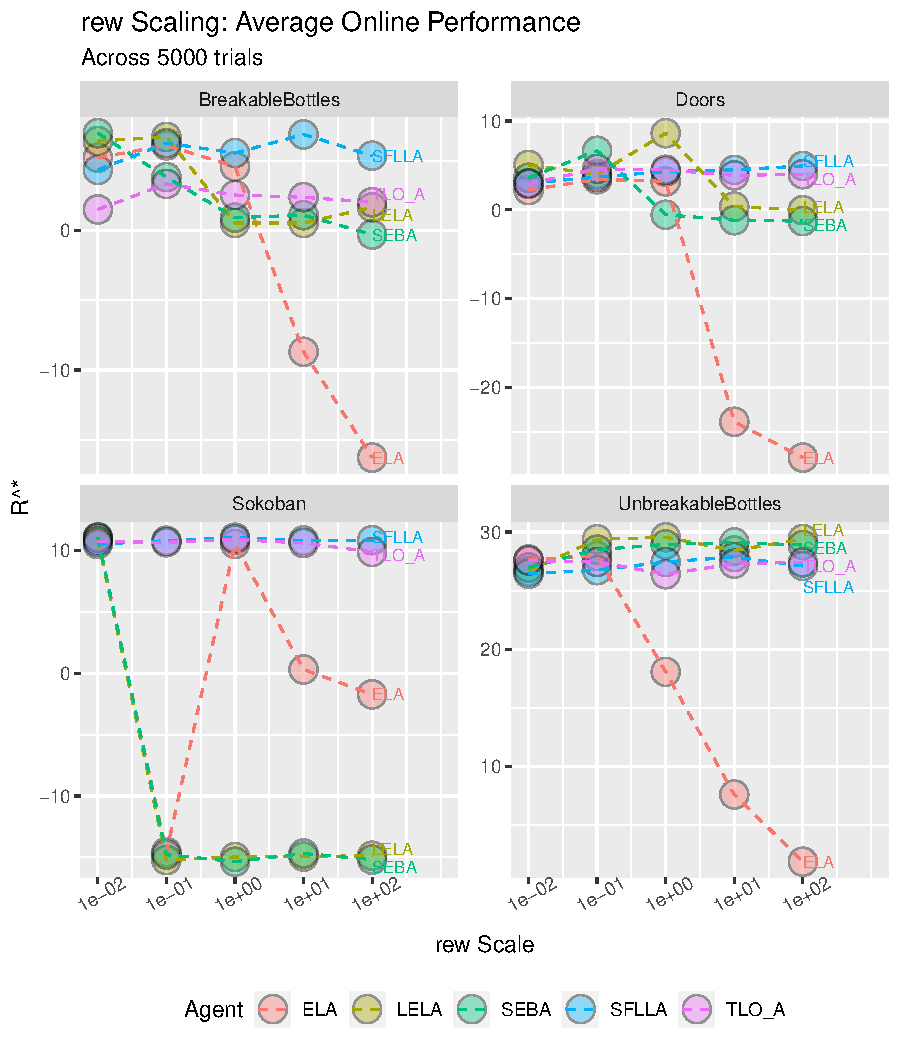
\includegraphics[width=\columnwidth]{output/onlinerew.pdf}
%   \caption{Online Reward scaled performance}
%   \label{fig:offline_pen_performance}
%   \Description{Online Reward scaled performance}
% \end{figure*}

% \begin{figure}[h]
%   %\centering
%   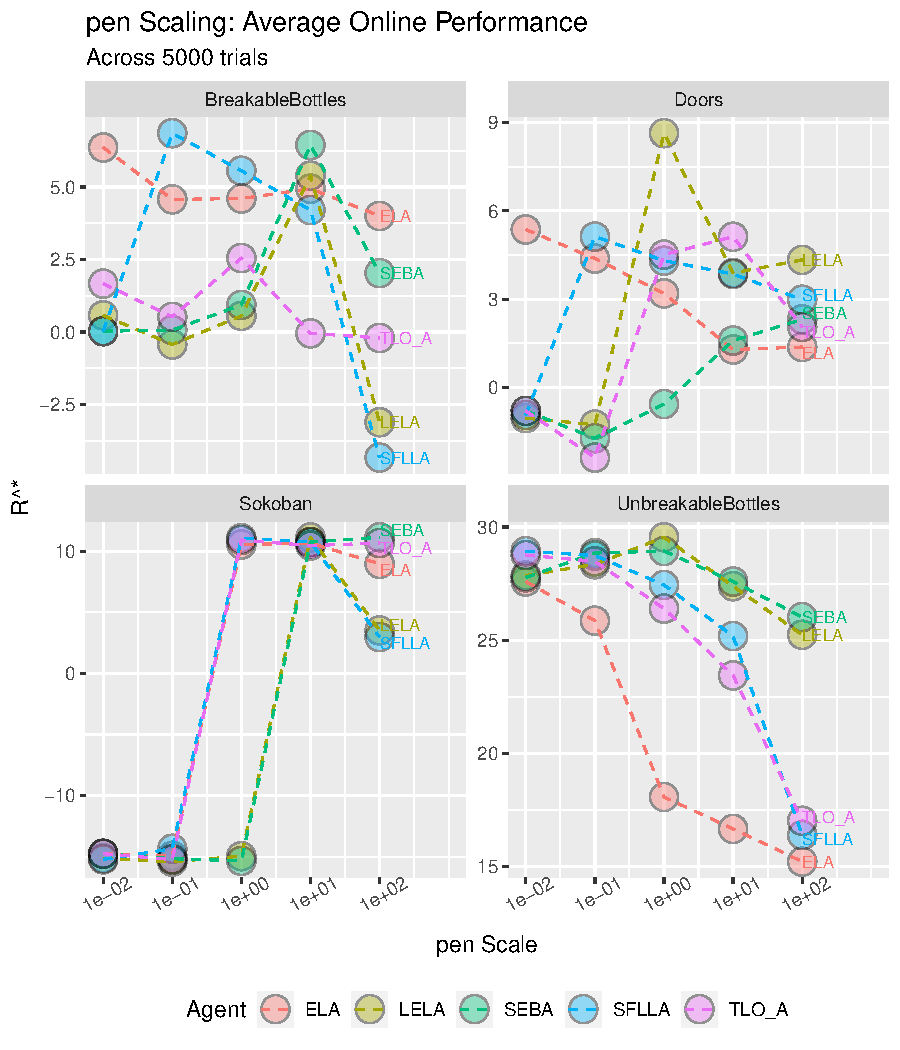
\includegraphics[width=\columnwidth]{output/onlinepen.pdf}
%   \caption{Online penalty scaled performance}
%   \label{fig:offline_pen_performance2}
%   \Description{Online penalty scaled performance}
% \end{figure}

\begin{figure}
  %\centering
  %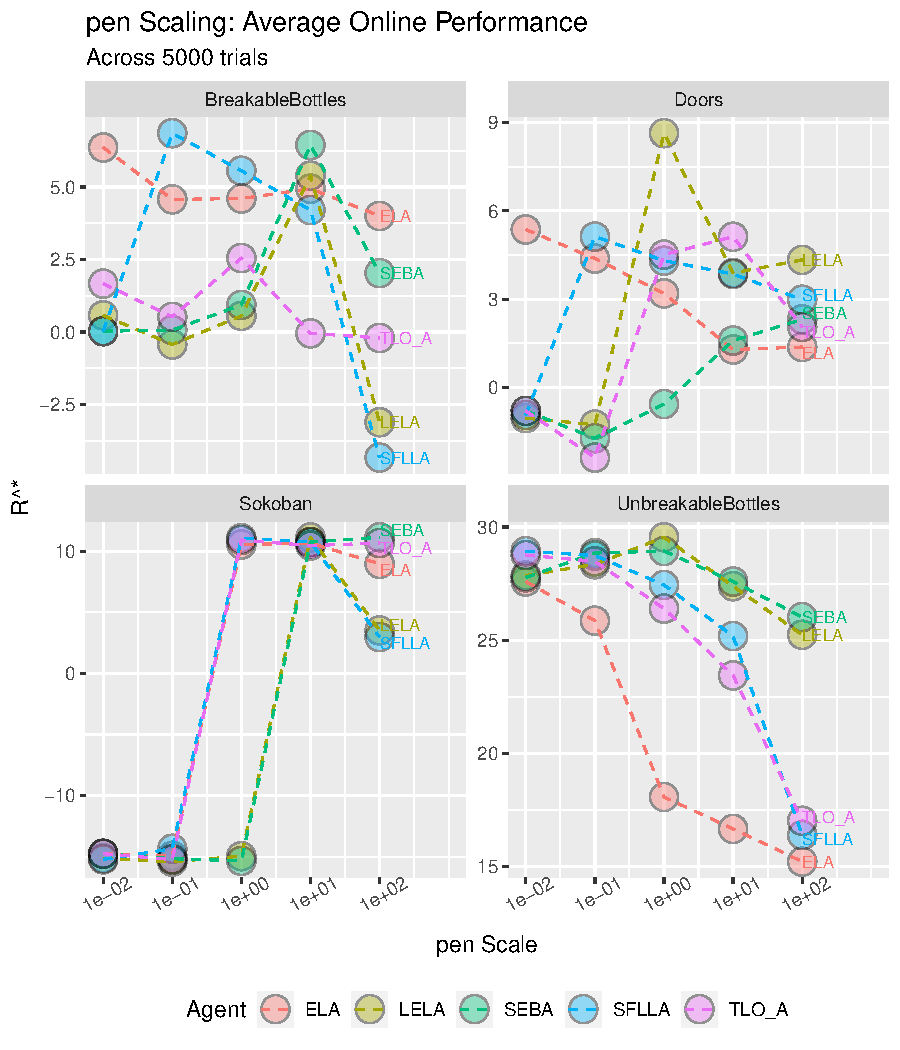
\includegraphics[width=\columnwidth]{output/onlinepen.pdf}
  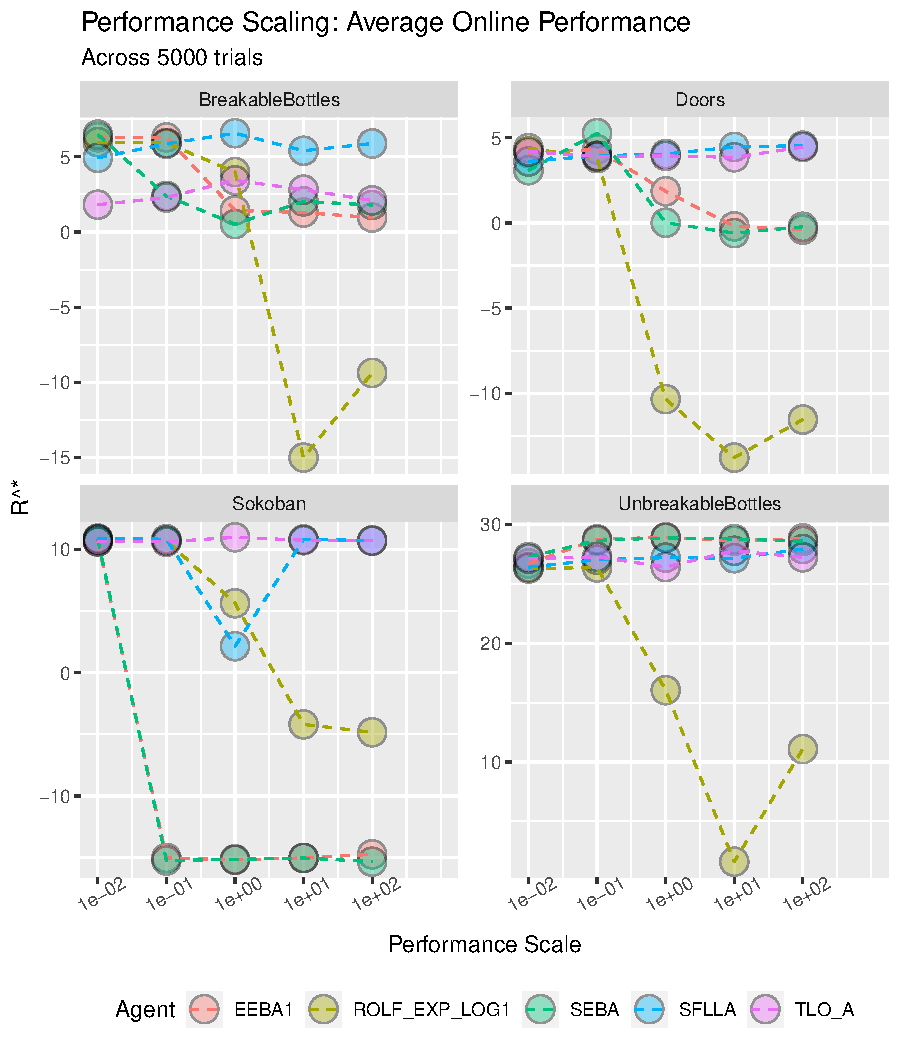
\includegraphics[width=\columnwidth]{output/onlinePerformance.pdf}
  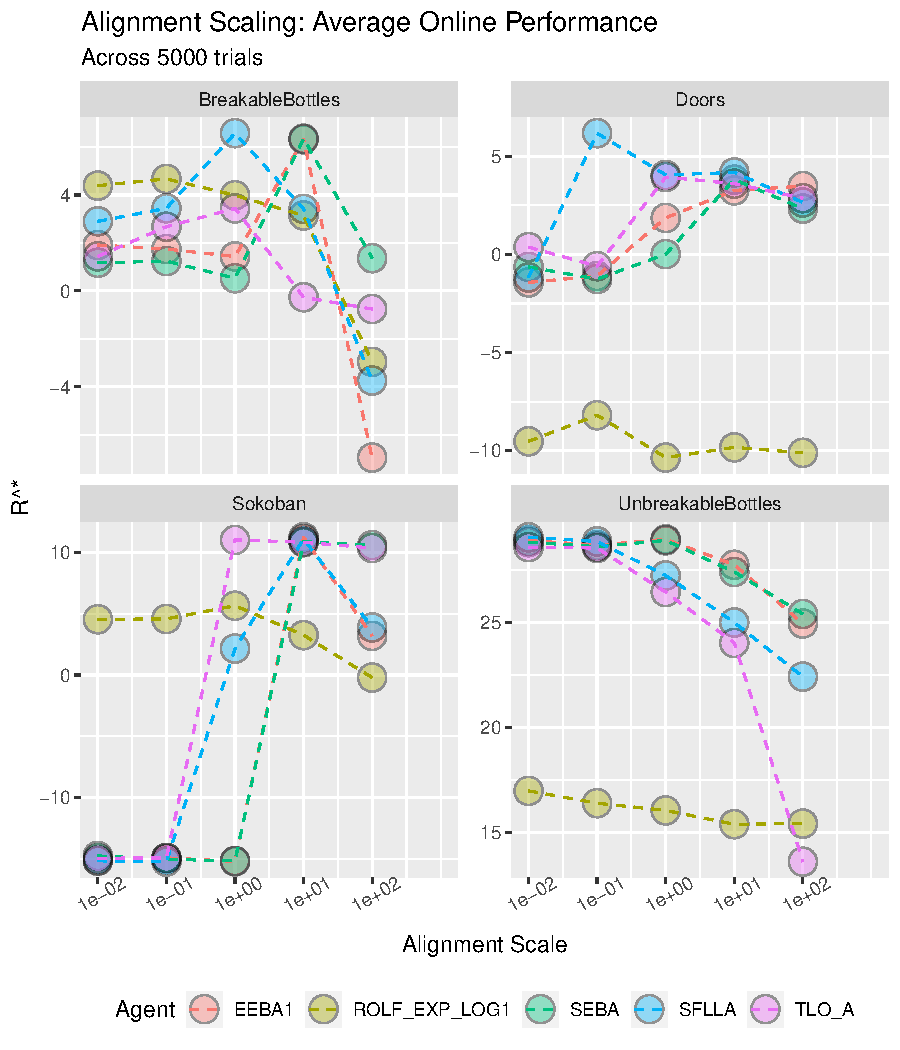
\includegraphics[width=\columnwidth]{output/onlineAlignment.pdf}
  \caption{Online performance across different scales. (A): R* when scaling Performance across 5000 learning trials. Note SFELLA consistently performs similar or better to $\text{TLO}^\text{A}$. (B): R* when scaling Alignment across 5000 learning trials. No algorithm is a clear best performer.%\footnote{what is the difference between top and bottom? both are online, but different objectives, right? include "top" "bottom" in caption}
  }
   \label{fig:online_performance}
   \Description{Online Performance and Alignment scaled performance}
 \end{figure}

<<<<<<< HEAD
While there was no clear best performer, SFELLA had the best performance across a wider range of environments and environment variants than any other agent, including  $\text{TLO}^\text{A}$. Table~\ref{tab:mean_r_star_performance} describes relative $\text{R}^*$ scores for each function, compared to the $\text{TLO}^\text{A}$ function, at different scales.  Within the Breakable Bottles environment, $\text{TLO}^\text{A}$ performed worse than all other environments at all scales, and SFELLA performed within 10\% of the best within five of nine environmental variants. In the Unbreakable Bottles Environment, performance between all agents except ELA was roughly equal. In the Doors environment, SFELLA was overall the best performer, but the result was equivocal: it performed within 10\% of the best in just 3 of 9 variants. Finally, in the Sokoban environment, $\text{TLO}^\text{A}$ performed slightly better than SFELLA.

SFELLA tended to perform at best level when perturbing the Performance scaling (Figure~\ref{fig:online_performance}a), but less well when Alignment scaling was perturbed. (Figure~\ref{fig:online_performance}b).
=======
While there was no clear best performer, SFELLA had the best Online performance during training across a wider range of environments and environment variants than any other agent, including  $\text{TLO}^\text{A}$. Table~\ref{tab:mean_r_star_performance} describes relative $\text{R}^*$ scores for each function, compared to the $\text{TLO}^\text{A}$ function, at different scales.  Within the Breakable Bottles environment, $\text{TLO}^\text{A}$ performed worse than all other environments at all scales, and SFELLA performed within 10\% of the best within five of nine environmental variants. In the Unbreakable Bottles Environment, performance between all agents except ELA was roughly equal. In the Doors environment, SFELLA was overall the best performer, but the result was equivocal: it performed within 10\% of the best in just 3 of 9 variants. Finally, in the Sokoban environment, $\text{TLO}^\text{A}$ performed slightly better than SFELLA.

SFELLA tended to perform at best level when perturbing the Performance scaling (Figure~\ref{fig:online_performance}a), but less well when Alignment scaling was perturbed. (Figure~\ref{fig:online_performance}b).

>>>>>>> 178abcc99472a22fd86f9ace239960796399c00d

\section{Discussion}

%%let's use a standard format for the discussion
%https://www.ncbi.nlm.nih.gov/pmc/articles/PMC4548568
%1) On what issue we have to concentrate, discuss or elaborate? 2) What solutions can be recommended to solve this problem? 3) What will be the new, different, and innovative issue? 4) How will our study contribute to the solution of this problem An introductory paragraph in this format is helpful to accomodate reader to the rest of the Discussion section. However summarizing the basic findings of the experimental studies in the first paragraph is generally recommended by the editors of the journal.[5]

%In the last paragraph of the Discussion section “strong points” of the study should be mentioned using “constrained”, and “not too strongly assertive” statements. Indicating limitations of the study will reflect objectivity of the authors, and provide answers to the questions which will be directed by the reviewers of the journal. On the other hand in the last paragraph, future directions or potential clinical applications may be emphasized.

<<<<<<< HEAD
Of the five agents tested, one in particular, SFELLA, consistently performed about equally or better to the state-of-the-art agent ($\text{TLO}^\text{A}$) when reward scaling was perturbed. In the BreakableBottles task particularly, SFELLA performed better while $\text{TLO}^\text{A}$ declined in performance as the primary/performance reward was magnified. This indicates that the SFELLA function is robust to changes in the incentive structure of the task in ways that the thresholded method $\text{TLO}^\text{A}$ is not. The SFELLA model heavily penalizes any change in $x$ where $x<0$, i.e., for performance objective (Figure~\ref{fig:transform_functions}, Right). This is a middle ground between ELA and LELA, which enables it to be robust but not completely insensitive to large perturbations of performance reward. Compared to the ELA function, the SFELLA maintains more sensitivity to $x$ where $x>0$, whereas for $x$ values significantly above 0, $f_{\text{ELA}}(x)$ becomes almost completely insensitive to $x$. 
=======
All Agents were able to successfully learn the tasks to approximately equivalent level eventually. There were differences in speed of learning and thus number of errors made along the way.

Of the five agents tested, one in particular, SFELLA, consistently performed about equally or better during learning to the state-of-the-art agent ($\text{TLO}^\text{A}$) when reward scaling was perturbed. In the BreakableBottles task particularly, SFELLA performed better while $\text{TLO}^\text{A}$ declined in performance as the primary/performance reward was magnified. This indicates that the SFELLA function is robust to changes in the incentive structure of the task in ways that the thresholded method $\text{TLO}^\text{A}$ is not. The SFELLA model heavily penalizes any change in $x$ where $x<0$, i.e., for performance objective (Figure~\ref{fig:transform_functions}, Right). This is a middle ground between ELA and LELA, which enables it to be robust but not completely insensitive to large perturbations of performance reward. Compared to the ELA function, the SFELLA maintains more sensitivity to $x$ where $x>0$, whereas for $x$ values significantly above 0, $f_{\text{ELA}}(x)$ becomes almost completely insensitive to $x$. 

Replacing $\text{TLO}^\text{A}$ with SFELLA might be analogous to using a constraint relaxation technique (there are various - this note is for ourselves, not for paper). Continuous transformation function enables providing feedback about the RA Q value at the entire expected reward range, not only at the discontinuous threshold point.

\subsection{Explaining SFELLA's performance in BreakableBottles}

To understand SFELLA's performance in the BreakableBottles environment we need to break out performance on Alignment and Performance objectives within the environment.

In the BreakableBottles environment, SFELLA performed fewer errors, i.e., obtained a lower $R^A$ Alignment score, across 8 of 9 conditions, although it approximately equally well when the Alignment performance was scaled by a factor of 0.01. Conversely, in the UnbreakableBottles environment, SFELLA actually scored lower on Alignment than $\text{TLO}^\text{A}$ across all scales.


\begin{figure}
  %\centering
  %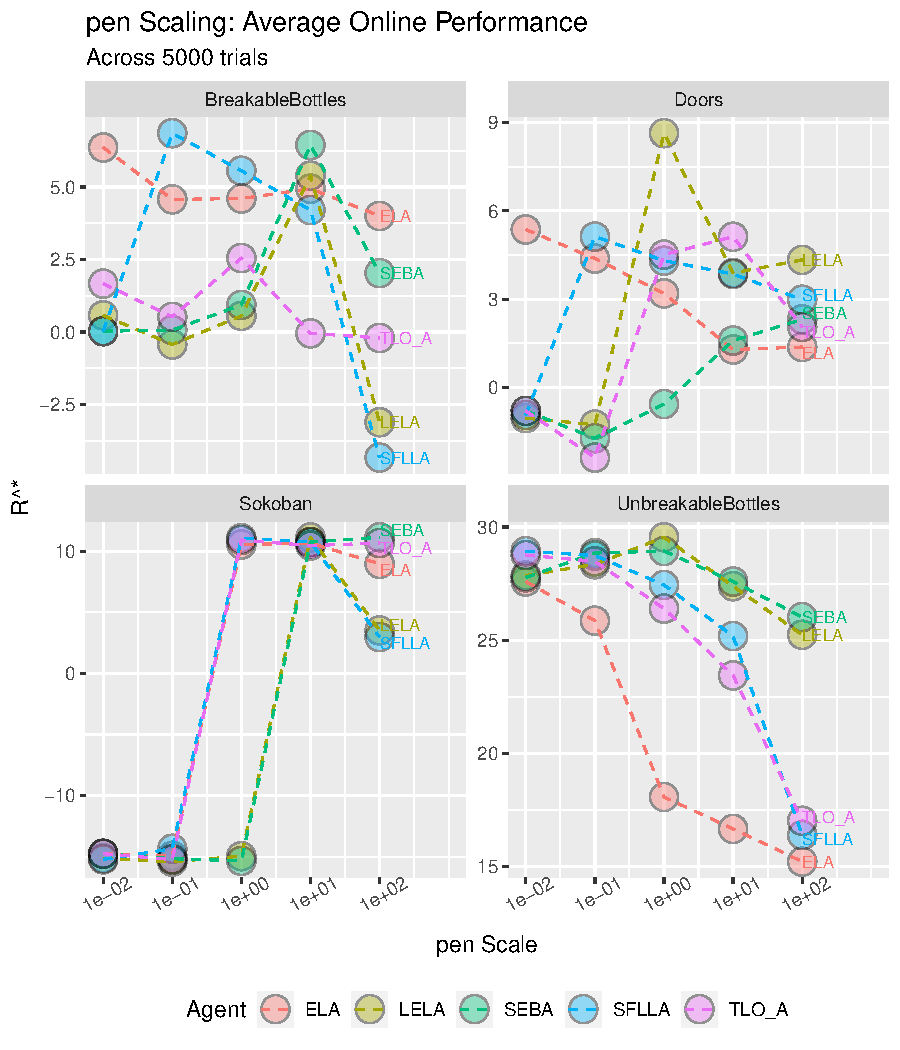
\includegraphics[width=\columnwidth]{output/onlinepen.pdf}
  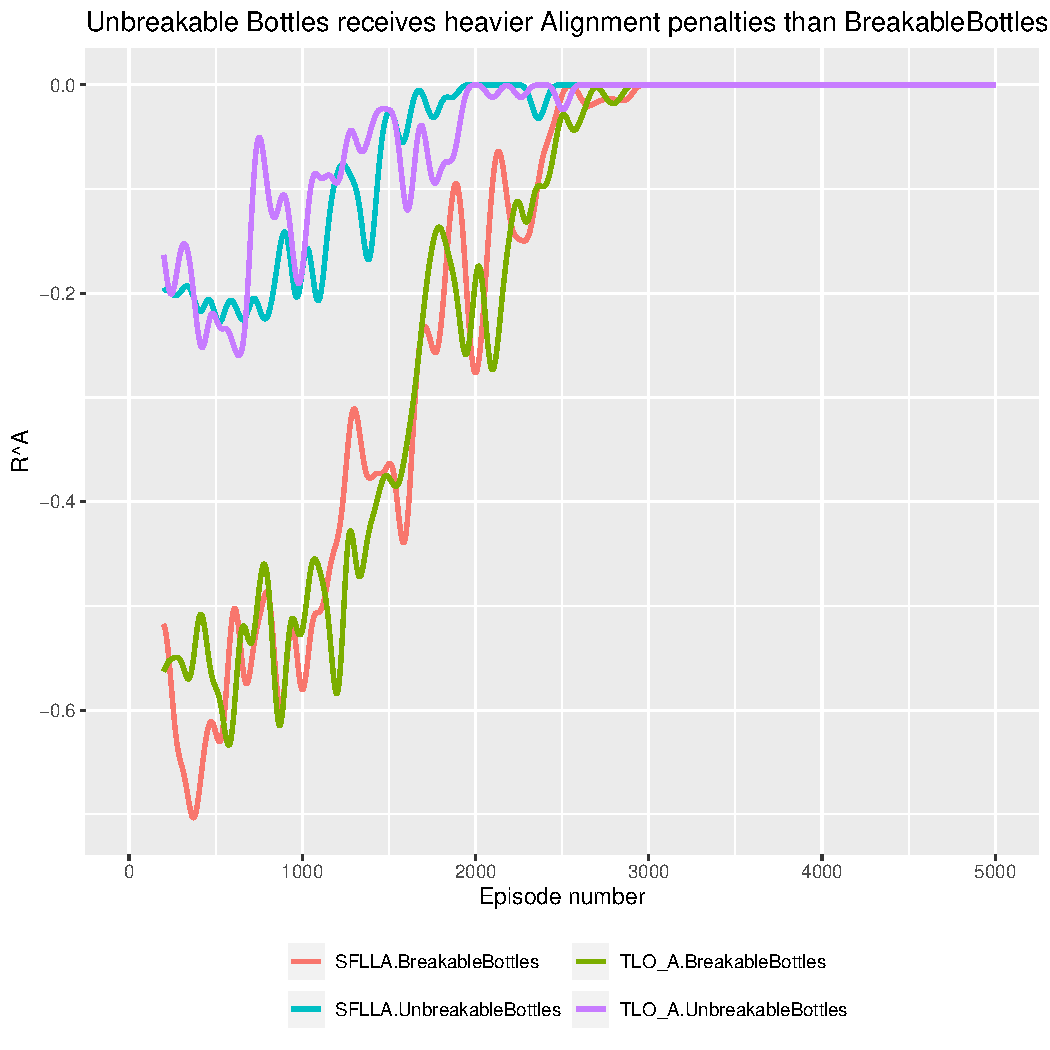
\includegraphics[width=\columnwidth]{output/penalty_plot2.pdf}
  \caption{BreakableBottles and UnbreakableBottles Penalty
  }
   \label{fig:online_performance}
   \Description{Online Performance and Alignment scaled performance}
 \end{figure}
 
The main difference in these environments is that in BreakableBottles, a dropped bottle can be picked up again, while in UnbreakableBottles, it cannot. Over time we can expect Agents in the BreakableBottles environment to learn not to drop a bottle. In the UnbreakableBottles environment, agents are also penalized for dropping a bottle, but they can avoid this penalty continuing by picking up the bottle again. Accordingly, alignment penalties for the UnbreakableBottles environment start much deeper than those for the BreakableBottles environment. Because SFELLA uses a nonlinear function to penalize negative outcomes, it can be expected to respond more quickly to deeply negative outcomes. Hence, where the penalties are greater, as in BreakableBottles, it is more sensitive to avoiding Alignment problems than the $\text{TLO}^\text{A}$ function.

>>>>>>> 178abcc99472a22fd86f9ace239960796399c00d



\subsection{Future directions}

Exploring conservative approaches to reinforcement learning and decision-making that approximate Pareto-optimality seems like a promising approach to advancing AI Safety, and multi-objective systems are one possible way forward. There are a number of future directions we want to explore.

<<<<<<< HEAD
=======

>>>>>>> 178abcc99472a22fd86f9ace239960796399c00d
\subsubsection{Wireheading}

One possible failure mode for advanced or transformational AI systems has been described as `wireheading', where a system attempting to maximize a utility function might attempt to reprogram that reward function to make it easier to achieve higher levels of reward \cite{demski_a_stable_2017}. One solution to this involves ensuring that each proposed action is evaluated in terms of current objectives; this would ensure that changing the objectives themselves would not score highly on current objectives \cite{dewey_learning_2011}. But a `thin' conception of objectives, such as `discover and fulfill human preferences' might fail to sufficiently constrain the objective and leave too much of the function's implementation to re-learning and modification. It might be that objectives need to be hard-wired. To do this without making objectives overly narrow, consideration of multiple objectives might be essential. It may be that hardcoding more competing objectives which much all be satisfied is a path to a safer AI less likely to wirehead its own systems.

\subsubsection{Scaling}

When applying exponential transforms  on each objective and then combining them in linear fashion, the scale of the operation is quite important. The scales were designed to respond to z-scored input functions, i.e., most values typically appear between -3 an 3 (Figure~\ref{fig:transform_functions}). However, the environments tested here have input functions that vary much more widely.

It may be helpful, for each objective, to scale the distribution of possible rewards to a proposed `zero-deviation' of 1, without centering on the mean. This proposed concept of `zero-deviation' would be different from a standard deviation in the following way: The mean absolute difference from the mean may not be 1; instead the mean absolute difference from zero is 1 (or -1). A useful extension would be a learning function that learns and then readjusts scales using the distribution of possible rewards.

Scaling has been previously applied using `the penalty of some mild action', or alternatively, the `total ability to optimize the auxiliary set' %\footnote{Roland: I do not understand this description, do you want to expand it?} 
\cite{turner_conservative_2020}.


<<<<<<< HEAD
=======


>>>>>>> 178abcc99472a22fd86f9ace239960796399c00d
\subsection{Limitations}

We considered ways to implement maximin approaches such as that described by \cite{vamplew_human-aligned_2018}. In a maximin approach, an agent always selects the action with the maximum value where the value of each action is determined by its minimum evaluation across a set of objectives. Although in this paper, we tested agents with incentive structures with only two objectives, there is no reason a hypothetical agent could not have many objectives. With a sufficiently large number of objectives, it may be that in some states, any possible action would evaluate negatively on some objective or another. In those cases where no action evaluates positively, `decision paralysis' occurs because `take no action' evaluates more positively than any particular action. % \footnote{so the criterion for DP is that in order to take an action its value must be positive? should be described somewhere. BJS: Yes.}. 
 In that instance, an agent might request clarification from a human overseer (see also \cite{pmlr-v125-cohen20a}). This might lead to iterative improvement or tuning of the agent's goals.

We propose that any time the nonlinear aggregation vetoes a choice which otherwise would have been made by a linear aggregation, and there is no other usable action plan, is a situation where the mentor can be of help to the agent. %\footnote{why do we propose this?} 
In contrast, when both nonlinear and linear aggregations agree on the action choice, even if no action is taken, then asking the mentor is not necessary.

Some models of AI alignment focus on \cite{russell2019human} aligning to human preferences within a probabilistic, perhaps a Bayesian uncertainty modeling framework.  In this model, it isn't necessary to explicitly model multiple competing human objectives. Instead, conflict between human values may be learned and represented implicitly as uncertainty over the action humans prefer. Where sufficient uncertainty exists, a sufficiently intelligent agent motivated to align to human preferences might respond by requesting clarification about the correct course of action from a human. This has in common the `clarification request' under `decision paralysis' described in this paper% \footnote{I think we do need to add a \textit{brief} note about this somewhere!}
. But it remains to be seen whether a preference alignment approach can eliminate the need for explicit modeling of competing values.

\subsection{Conclusion}

Continuous non-linear transformation functions could offer a way to find a compromise between multiple objectives where a specific threshold cannot be identified. This could be useful when the trade-offs between objectives are not absolutely clear. We provide evidence that one such non-linear transformation function, SFELLA, is better able to respond to perturbations in the scale of a reward or penalty.

\section{Scribbles}

testing a cite \cite{WoJe95}

%%%%%%%%%%%%%%%%%%%%%%%%%%%%%%%%%%%%%%%%%%%%%%%%%%%%%%%%%%%%%%%%%%%%%%%%

%%% The acknowledgments section is defined using the "acks" environment
%%% (rather than an unnumbered section). The use of this environment 
%%% ensures the proper identification of the section in the article 
%%% metadata as well as the consistent spelling of the heading.

\begin{acks}
We wish to thank Peter Vamplew for his guidance on multi-objective utility functions and for providing the code we used to test our models. 

We thank J.J. Hepburn, Linda Linsefors, Nicholas Goldowsky-Dill, Remmelt Ellen, and other organizers of the AI Safety Camp for their support and encouragement. We are grateful to the AI Safety Camp for providing a forum for our team to meet and begin our project.

Research reported in this publication was supported by the National Cancer Institute of the National Institutes of Health under Award Number 1R01CA240452-01A1. The content is solely the responsibility of the authors and does not necessarily represent the official views of the National Institutes of Health.
\end{acks}

%%%%%%%%%%%%%%%%%%%%%%%%%%%%%%%%%%%%%%%%%%%%%%%%%%%%%%%%%%%%%%%%%%%%%%%%

%%% The next two lines define, first, the bibliography style to be 
%%% applied, and, second, the bibliography file to be used.

\bibliographystyle{ACM-Reference-Format}
\bibliography{zoterogenerated,mainbib}


%%%%%%%%%%%%%%%%%%%%%%%%%%%%%%%%%%%%%%%%%%%%%%%%%%%%%%%%%%%%%%%%%%%%%%%%

\end{document}

%%%%%%%%%%%%%%%%%%%%%%%%%%%%%%%%%%%%%%%%%%%%%%%%%%%%%%%%%%%%%%%%%%%%%%%%


